\documentclass[10pt]{beamer}

\usepackage{../macros}
\usetikzlibrary{shapes,arrows, chains}
\usepackage{ulem}
\title{Itérations (while)}

\hypersetup{
  pdftitle =  {Itérations (while)}
}

\metroset{sectionpage=progressbar,subsectionpage=progressbar}


\begin{document}

\maketitle

%%%%%%%%%%%%%%%%%%%%%%%%%%%%%%%%%%%%%%%%%%%%%%%%%%%%%%%
\begin{frame}
  \frametitle{Problème $\rightarrow$ Algorithme $\rightarrow$ Programme}

  
  \begin{itemize}
  \item Partons d'un \alert{problème}.
  \item Soit à faire calculer la somme des entiers de $[1,n]$, avec $n$ entier $\geq 1$.
    \[
      S = 1 + 2 + 3 + \ldots + n-1 + n
    \]
  \item Cette somme S dépendant de $n$, intéressons-nous à la fonction $S(n)$.
    \[
      S(n) = 1 + 2 + 3 + \ldots + n-1 + n = \sum_{i=1}^n i
    \]
  \item Il s'agit de construire un \alert{algorithme} de calcul de $S(n)$ : une \alert{méthode mécanique} permettant d'arriver au résultat.
  \item Une fois un tel algorithme obtenu, il s'agira de coder la fonction $S$ dans un langage de programmation, ici R.
  \item Pour produire au final un \alert{programme exécutable} sur machine.
  \end{itemize}

\end{frame}

%%%%%%%%%%%%%%%%%%%%%%%%%%%%%%%%%%%%%%%%%%%%%%%%%%%%%%%
\begin{frame}
  \frametitle{Calculs répétitifs}

  \begin{block}{Je veux calculer $S(1000)$}
    Faire le calcul à la main est facile, long et prodigieusement ennuyeux : $1 + 2 + 3 + 4 + 5 + 6 +7 + \ldots + 1000$. Ouf.
  \end{block}
  
  \begin{block}{Je ne veux pas FAIRE le calcul}
    je veux le FAIRE FAIRE par un ordinateur (computer). \\
    Il me faut donc écrire un programme court qui explique à la machine par quelles étapes passer. 
    La taille du programme ne dépendra pas de $n$, mais le temps de calcul probablement.
  \end{block}
  
  \begin{alertblock}{Trois méthodes classiques pour construire un algorithme}
    \begin{itemize}
    \item Le \alert{\textbf{calcul direct}}.
    \item La \alert{\textbf{récurrence}}.
    \item La \alert{\textbf{boucle}}.
    \end{itemize}
  \end{alertblock}
\end{frame}

%%%%%%%%%%%%%%%%%%%%%%%%%%%%%%%%%%%%%%%%%%%%%%%%%%%%%%%
\begin{frame}[fragile]
  \frametitle{Les calculs répétitifs : CALCUL DIRECT !}
  Rarement possible, demande souvent un peu d'astuce, comme celle de Gauss vers ses 14 ans :
  \begin{table}[h]
    \centering
    \begin{tabular}{r@{ $=$ }*{5}{c@{ $+$ }}c}
      $S(n)$          & $1$     & $2$     & $3$     & $\ldots$ & $n-1$   & $n$ \\
      $S(n)$          & $n$     & $n-1$   & $n-2$   & $\ldots$ & $2$     & $1$ \\
      \midrule
      $2 \times S(n)$ & $n + 1$ & $n + 1$ & $n + 1$ & $\ldots$ & $n + 1$ & $n + 1$ 
                                                                                  
    \end{tabular}
  \end{table}
  
  \begin{block}{En R}
  \begin{lstlisting}[style=block]
> S <- function(n) {return(n*(n+1)/2)}
> paste('S(1000)=', S(1000))
[1] S(1000) = 500500   
\end{lstlisting}
\begin{itemize}
\item La taille du programme (longueur de son texte) ne dépend pas de \texttt{n}, qui ne sera fourni qu'à l'exécution.
\item Le temps d'exécution du calcul de \texttt{S(1000)} est immédiat. \\
  Il coûte 3 opérations.
\end{itemize}
  \end{block}
\end{frame}


%%%%%%%%%%%%%%%%%%%%%%%%%%%%%%%%%%%%%%%%%%%%%%%%%%%%%%%
\begin{frame}[fragile]
  \frametitle{Les calculs répétitifs : RECURRENCE}
  \only<1>{
    Appréciée des matheux, elle permet souvent d'attaquer des problèmes difficiles en \dots supposant le problème résolu !

  Il s'agit de réduire le problème $S(n)$ à un problème $S(k)$ avec $k < n$.
  On prend souvent $k = n-1$ ou $n \div 2$. On remarque ici que pour $n > 0$ :
  \[
    S(n) = \underline{(1 + 2 + 3 + \ldots + n-1)} + n = S(n-1) + n
  \]
  Si l'on sait calculer $S(n-1)$, on sait donc calculer $S(n)$.
  Or on sait calculer $S(1) = 1$, d'où un calcul de proche en proche :
  \[
    S(2) = S(1) + 2 = 3 \qquad     S(3) = S(2) + 3 = 6 \qquad S(4) = S(3) + 4 = 10      
  \]
  }
  
\begin{lstlisting}[style=edblock]
S <- function(n) {
  if( n <= 0) return(0)
  else return( S(n-1) + n )
}
\end{lstlisting}    

\only<2>{
\begin{itemize}
\item La taille du programme ne dépend toujours pas de \texttt{n}, qui ne sera fourni qu'à l'exécution.
\item Le \alert{temps} d'exécution du calcul de \texttt{S(1000)} est \alert{linéaire}. \\
  Il coûte n-1 opérations.
\end{itemize}
}

\begin{block}<2>{R n'encourage pas la récurrence et ne l'optimise pas !}
  \begin{lstlisting}[style=block]
> S(1000)
Erreur : évaluations trop profondément imbriquées : récursion infinie / ...    
  \end{lstlisting}
\end{block}

\end{frame}

%%%%%%%%%%%%%%%%%%%%%%%%%%%%%%%%%%%%%%%%%%%%%%%%%%%%%%%
\begin{frame}
  \frametitle{ Les calculs répétitifs : BOUCLES}
  Plus populaire chez les programmeurs, elle tâche de présenter le calcul comme une succession d'étapes identiques portant sur des variables qui changent de valeur à chaque étape.

  \begin{alertblock}{L'important est la situation et non l'action.}
    
\begin{columns}[t]
\begin{column}{0.43\textwidth}
  \begin{itemize}
  \item \sout{Qu'allons-nous faire ?}
  \item \sout{Comment procéder ?}
  \end{itemize}
\end{column}
\begin{column}{0.57\textwidth}
  \begin{itemize}
  \item Où en sommes-nous ?
  \item Quelle est la situation générale ?
  \end{itemize}
\end{column}
\end{columns}

  \end{alertblock}

  \begin{itemize}
\item J'ai commencé à calculer $S(n)$. En plein milieu du calcul, où en suis-je ?
\item Par exemple, j'ai déjà calculé $1 + 2 + 3 + \ldots + \mathtt{i}$.
Introduisons une variable $\mathtt{acc}$ représentant cette accumulation.
Nous gérons donc deux variables $\mathtt{i}$ et $\mathtt{acc}$.
\end{itemize}

  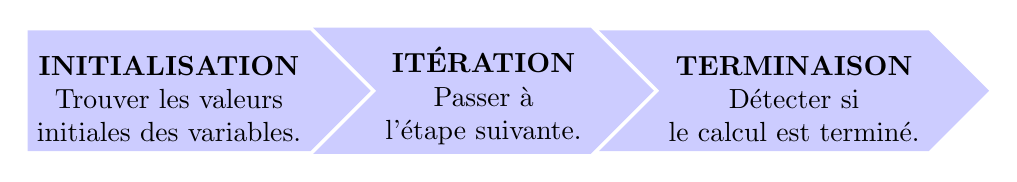
\begin{tikzpicture}
    \begin{scope}[start chain,node distance=0.5mm, every node/.style={on chain, draw=none, shape=signal, align=center, fill=blue!20, text height =1.3cm}] 
  \node(INI)  {\textbf{INITIALISATION}\\Trouver les valeurs\\initiales des variables.};
  \node(ITER) [signal from=west]  {\textbf{ITÉRATION}\\Passer à\\l’étape suivante.};
  \node(TERM) [signal from=west] {\textbf{TERMINAISON}\\Détecter si\\le calcul est terminé.};
    \end{scope}
  \end{tikzpicture}
\end{frame}


%%%%%%%%%%%%%%%%%%%%%%%%%%%%%%%%%%%%%%%%%%%%%%%%%%%%%%%

\begin{frame}{Construire une itération}
  Une fois la situation générale trouvée, voici les trois temps de la construction d'une itération :
  \begin{block}{Passer à l'étape suivante (\alert{ITÉRATION})}
    Étant en possession de $\mathtt{acc} = 1 + 2 + \dots + \mathtt{i}$, on voudra obtenir la valeur de $1 + 2 + \ldots + \mathtt{i} + (\mathtt{i}+1)$. Il suffira donc d'ajouter $\mathtt{i}+1$ à $acc$ et d'ajouter 1 à $\mathtt{i}$.    
  \end{block}
  \begin{block}{Détecter si le calcul est terminé (\alert{TERMINAISON})}
    On aura terminé lorsque $\mathtt{i}$ sera égal à $n$ puisqu'alors $\mathtt{acc}$ vaudra $S(n)$.
  \end{block}

  \begin{block}{Trouver les valeurs initiales des variables (\alert{INITIALISATION})}
    Au début du calcul, je peux prendre $\mathtt{i} = 1$ et $\mathtt{acc} =1$. \\
    Je pourrais aussi prendre $\mathtt{i} = 0$ et $\mathtt{acc} = 0$ \dots \\
    Le tout, c'est que ma situation générale $\mathtt{acc} = 1 + 2 + \ldots + \mathtt{i}$ soit vraie en début de boucle.
  \end{block}
  Si l'une de ces étapes s'avère trop difficile, il faudra envisager de trouver une autre situation générale
\end{frame}
%%%%%%%%%%%%%%%%%%%%%%%%%%%%%%%%%%%%%%%%%%%%%%%%%%%%%%%
\def\circledarrow#1#2#3{ % #1 Style, #2 Center, #3 Radius
\draw[#1,->] (#2) +(80:#3) arc(80:-260:#3);
}
\begin{frame}[fragile]
  \frametitle{Visualiser une boucle}
  \tikzstyle{block} = [draw, fill=blue!20, rectangle, minimum height=3em, minimum width=6em]
\tikzstyle{sum} = [draw, fill=red!20, circle]
%\tikzstyle{input} = [coordinate]
\tikzstyle{output} = [coordinate]
\tikzstyle{pinstyle} = [pin edge={to-,thin,black}]

% The block diagram code is probably more verbose than necessary
\begin{tikzpicture}[auto, node distance=2cm,>=latex']
    % We start by placing the blocks
    \node [block, align = left] (INIT) {$\mathtt{i} = 0$\\$\mathtt{acc}=0$};
    \node [sum, right of=INIT, node distance=2cm] (INV) {INV};
    \node [block, diamond, right of=INV, , node distance=2cm] (TERM) {$\mathtt{i} == n$ ?};
    \node [block, right of=TERM, align = left, node distance=4cm] (END) {FIN\\Le résultat est $\mathtt{acc}$.};
    % We draw an edge between the TERM and END block to 
    % calculate the coordinate u. We need it to place the measurement block. 
    %\node [output, right of=END] (output) {};
    \node [block, align = left, below of=TERM, node distance=2cm] (ITER) {$\mathtt{i} = \mathtt{i} + 1$\\$\mathtt{acc}=\mathtt{acc}+\mathtt{i}$};

    % Once the nodes are placed, connecting them is easy. 
    \draw [draw,->] (INIT) -- (INV);
    \draw [->, ultra thick] (INV) -- (TERM);
    \draw [->, ultra thick] (TERM) -- node {\texttt{FALSE}} (ITER);
    \draw [->, ultra thick] (ITER) -| (INV);
    \draw [->] (TERM) -- node {\texttt{TRUE}} (END);

      \end{tikzpicture}

    À chaque entrée dans la boucle, au point INV, la situation générale $\mathtt{acc} = 1 + 2 + \dots + \mathtt{i}$ est vérifiée !

\begin{columns}[c]
\begin{column}{0.48\textwidth}
  On boucle tant que $\mathtt{i} < n$.
  Une des manières d'exprimer une boucle consiste à utiliser le mot-clé \texttt{while} qui signifie "tant que".
\end{column}
\begin{column}{0.48\textwidth}
\begin{lstlisting}[style=editor]
S <- function(n) {
  i <- 0
  acc <- 0
  while(i < n) {
    i <- i + 1
    acc <- acc + i
  }
  return(acc)
}  
\end{lstlisting}
\end{column}
\end{columns}
\end{frame}
%%%%%%%%%%%%%%%%%%%%%%%%%%%%%%%%%%%%%%%%%%%%%%%%%%%%%%%
\begin{frame}[fragile]
  \frametitle{Commutation d'instructions}
\begin{alertblock}{MISE EN GARDE : deux instructions ne commutent pas en général.}
  Les deux suites d’instructions ci-dessous ne sont PAS équivalentes. 
\end{alertblock}

  
\begin{columns}[c]
  \begin{column}{0.25\textwidth}
  \begin{lstlisting}[style=editor]
i <- i + 1 
acc <- acc + i 
  \end{lstlisting}
\end{column}
\begin{column}{0.25\textwidth}
  \begin{lstlisting}
i = 2
acc = 3
\end{lstlisting}
\end{column}
\begin{column}{0.1\textwidth}
  \RUN
\end{column}
\begin{column}{0.25\textwidth}
  \begin{lstlisting}
i = 3
acc = 6
\end{lstlisting}
\end{column}
\end{columns}

Cette suite d'instruction serait fausse.
\begin{columns}[c]
  \begin{column}{0.25\textwidth}
  \begin{lstlisting}[style=editor]
acc <- acc + i 
i <- i + 1
\end{lstlisting}
\end{column}
\begin{column}{0.25\textwidth}
  \begin{lstlisting}
i = 2
acc = 3
\end{lstlisting}
\end{column}
\begin{column}{0.1\textwidth}
  \RUN
\end{column}
\begin{column}{0.25\textwidth}
  \begin{lstlisting}
i = 3
acc = 5
\end{lstlisting}
\end{column}
\end{columns}

Il s'agit d'un point noir des boucles dans les langages impératifs.

\begin{alertblock}{Deux instructions peuvent commuter si elles sont indépendantes.}
Or ci-dessus, l'affectation de \texttt{i} modifie la valeur de \texttt{i} dans l'affectation de \texttt{acc}.
\end{alertblock}


\begin{block}{Problème important à l'heure des processeurs à plusieurs c{\oe}urs.}
 Si chaque c{\oe}ur modifie des variables \dots
\end{block}

\end{frame}


\begin{frame}[fragile]
  \frametitle{Mise au point ou debuggage}
  Il arrive aux meilleurs programmeurs de produire des programmes incorrects.
  \begin{alertblock}{Comment puis-je m'aider à détecter une erreur ?}
    Réponse : en espionnant la boucle \dots
  \end{alertblock}

  \begin{block}{La méthode classique du \texttt{printf}}
    On fait afficher les variables de boucle (les variables qui varient dans la boucle), ici \texttt{acc} et {i}. \alert{Observe-t-on une anomalie ?}   
  \begin{lstlisting}
while (i < n) {
  paste('i =',i,'acc =',acc)
  ...
\end{lstlisting}

\end{block}

    \begin{block}{La méthode plus avancée du \texttt{browser}}
      La fonction \texttt{browser} interrompt l'exécution de votre programme et permet l'inspection de l'environnement d'où a été appelée \texttt{browser}.
  \begin{lstlisting}
while (i < n) {
  browser()
  ...
\end{lstlisting}
\end{block}
\end{frame}


\begin{frame}
  \frametitle{Comment savoir si un nombre est premier}
Les nombres premiers 2, 3, 5, 7, 11... jouent un rôle important dans les codes secrets (cartes bancaires, mots de passe, etc).

Un entier $n$ est toujours divisible par $1$ et $n$, qui sont ses diviseurs triviaux.
Par exemple 12 est divisible par 1 et 12 (et par d'autres) \dots

Un entier $n$ est premier s'il est $\geq 2$ et si ses seuls diviseurs sont les diviseurs triviaux.
Par exemple 13 est premier, mais pas 12.

\begin{block}{Test de primalité (algotihme naïf)}
  Pour savoir si un nombre $n \geq 2$ est premier, il suffit donc d'examiner les nombres entiers $d$ de $[2,n-1]$ à la recherche d'un diviseur de $n$.
  \begin{itemize}
  \item Si l'on en trouve un, on s'arrête au premier avec le résultat \texttt{FALSE}.
  \item Sinon, le résultat sera \texttt{TRUE}.  

  \end{itemize}
\end{block}

\begin{block}{Quelle est la situation générale ?}
 J'en suis au nombre $d$ que je n'ai pas encore examiné, et je n'ai toujours pas trouvé de diviseur.  
\end{block}
\end{frame}
%%%%%%%%%%%%%%%%%%%%%%%%%%%%%%%%%%%%%%%%%%%%%%%%%%%%%%%
\begin{frame}[fragile]{Implémentation du test de primalité}
  \begin{lstlisting}[style=editor]
estPremier <- function(n) {
  if(n < 2) return(FALSE) # 0 et 1 ne sont pas premiers
  d <- 2 #le premier diviseur non trivial
  while( d < n) {
    if( n %% d == 0) return(FALSE) # Échappement
    d <- d + 1
  }
  return(TRUE)
}    
\end{lstlisting}

\begin{lstlisting}
> paste('2001 est premier:', estPremier(2001))
[1] "2001 est premier: FALSE"  
> paste('2003 est premier:', estPremier(2003))
[1] "2003 est premier: TRUE"
\end{lstlisting}

\begin{alertblock}{Quel est le nombre d'opérations de notre test de primalité ?}
  \begin{lstlisting}[style=edblock]
> estPremier(.Machine$integer.max)   
\end{lstlisting}
% $ % for auctex
Ctrl-D ou Ctrl-C (Keyboard interrupt)
\end{alertblock}
\end{frame}

%%%%%%%%%%%%%%%%%%%%%%%%%%%%%%%%%%%%%%%%%%%%%%%%%%%%%%%
\begin{frame}[fragile]
  \frametitle{Les boucles infinies et l'instruction break}
  
  \begin{block}{Boucle \texttt{while}}
\begin{columns}[c]
\begin{column}{0.68\textwidth}
    Il est essentiel de s'assurer que la boucle termine, donc que le \texttt{<test>} finit par prendre la valeur \texttt{FALSE} .
  Sinon le programme entre dans une \alert{boucle infinie} et \dots on perd la main, il plante !

\end{column}
\begin{column}{0.38\textwidth}
  \begin{lstlisting}[style=editor]
while (<test>) {
<instruction>
<instruction>
...
}    
  \end{lstlisting}
\end{column}
\end{columns}
\end{block}

  \begin{block}{Boucle \texttt{repeat}}
\begin{columns}[c]
\begin{column}{0.68\textwidth}
  Pourtant certains programmeurs optent pour un style de boucle infinie dans lequel la décision d'échappement est prise parmi les instructions du corps de la boucle avec l'instruction \texttt{break}.
\end{column}
\begin{column}{0.38\textwidth}
  \begin{lstlisting}[style=editor]
repeat {
  <instruction>
  <instruction>
  ...
}    
  \end{lstlisting}
\end{column}
\end{columns}

  \end{block}
\begin{columns}[c]
\begin{column}{0.33\textwidth}
  \begin{lstlisting}[style=editor]
x <- 1
while(x <= 5) {
  x <- x +1
}    
\end{lstlisting}
\end{column}
\begin{column}{0.08\textwidth}
  $\Longleftrightarrow$
\end{column}
\begin{column}{0.33\textwidth}
\begin{lstlisting}[style=editor]
x <- 1
repeat {
  if(x > 5) break
  x <- x +1
}  
\end{lstlisting}

\end{column}
\end{columns}

\end{frame}

%%%%%%%%%%%%%%%%%%%%%%%%%%%%%%%%%%%%%%%%%%%%%%%%%%%%%%%
\begin{frame}[fragile]
  \frametitle{Boucle \texttt{repeat}}
\begin{columns}[c]
\begin{column}{0.63\textwidth}
  L'instruction break provoque une sortie brutale de la boucle, mais le programme continue son exécution après la boucle !
\end{column}
\begin{column}{0.33\textwidth}
  \begin{lstlisting}[style=edblock]
repeat {
  <instr>
  if (x > 5) break
  <instr>
}
# reprise ici 
\end{lstlisting}
\end{column}
\end{columns}



Quel intérêt ? Il se trouve que certaines boucles de ce type vont avoir le test de sortie en milieu ou en fin de boucle.
Il pourrait même y avoir plusieurs tests de sortie \dots

\begin{columns}[c]
\begin{column}{0.48\textwidth}
\begin{lstlisting}[style=editor]
x <- 1
repeat {
  if(x %% 11 == 0) break
  if(x %% 17 == 0) break
  x <- 2 * x +1
  print(x)
}  
\end{lstlisting}

\end{column}
\begin{column}{0.1\textwidth}
  \RUN
\end{column}

\begin{column}{0.28\textwidth}
  \begin{lstlisting}
[1] 3
[1] 7
[1] 15
[1] 31
[1] 63
[1] 127
[1] 255    
  \end{lstlisting}
\end{column}
\end{columns}
Cette boucle est donc la plus générale mais elle suppose que l'on garantisse bien sa terminaison, sinon GARE !
\end{frame}

%%%%%%%%%%%%%%%%%%%%%%%%%%%%%%%%%%%%%%%%%%%%%%%%%%%%%%%
 \questionSlide

%%%%%%%%%%%%%%%%%%%%%%%%%%%%%%%%%%%%%%%%%%%%%%%%%%%%%%%
 \appendix
 \backupSlides
%%%%%%%%%%%%%%%%%%%%%%%%%%%%%%%%%%%%%%%%%%%%%%%%%%%%%%%

%%%%%%%%%%%%%%%%%%%%%%%%%%%%%%%%%%%%%%%%%%%%%%%%%%%%%%%
% \begin{frame}[fragile]{Backup slides}
%   Sometimes, it is useful to add slides at the end of your presentation to
%   refer to during audience questions.

%   The best way to do this is to include the \verb|appendixnumberbeamer|
%   package in your preamble and call \verb|\appendix| before your backup slides.

%   will automatically turn off slide numbering and progress bars for
%   slides in the appendix.
% \end{frame}


%%%%%%%%%%%%%%%%%%%%%%%%%%%%%%%%%%%%%%%%%%%%%%%%%%%%%%%
% \begin{frame}[allowframebreaks]{References}

%   % \bibliography{../bib_parallelism,../bib_others}
%   % \bibliographystyle{abbrv}

% \end{frame}

\end{document}

%%% Local Variables:
%%% mode: latex
%%% TeX-master: t
%%% End:
